%!TeX root=Dissertation.tex
\section{Background}
%Desktop app. Analyse website log files. Outputs how risky the IPs are based on a variety of factors. A high risk level on an IP means it should probably be blocked. Risky IPs could carry out further attacks on the website and ultimately take it down. This can lead to loss of income and reputation for website owners. Aimed at website owners with little technical knowledge. 

The product that this project will produce will be a small desktop application capable of analysing large sets of website log data for website owners in a convenient way. Every time a website gets a visitor various properties of their visit are recorded in the log files, for example their IP, the access time, the type of HTTP request sent by the visitor, and the user agent. These files can therefore become quite large and difficult to read. This is a lot of potentially useful data that website owners could miss out on; it is important to analyse these files so that attacks can be identified. It is now even easier for anyone to own their own website (see figure \ref{Number of Websites}), but there are very few solutions available for analysing web traffic.

\begin{figure}[H] \label{Number of Websites} 
    \centering
    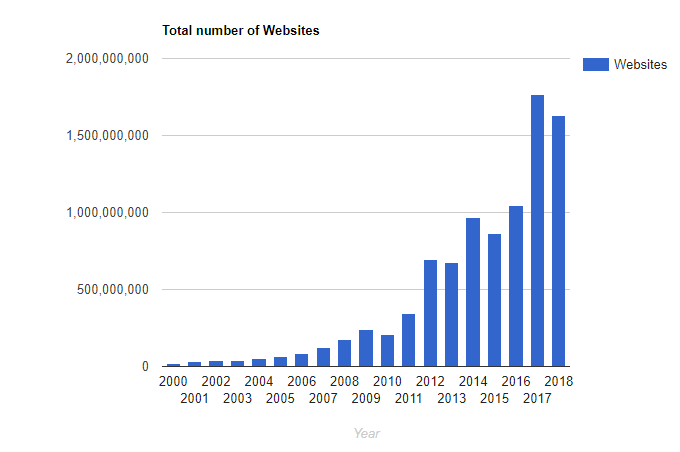
\includegraphics[width=\textwidth]{Images/numberOfWebsites.png}
    \caption{Total number of websites since 2000 (\cite{NumberofWebsites})}
    \label{Total number of websites since 2000}
\end{figure}
The majority of website owners are single individuals or small teams [REF] that do not necessarily have the time or resources to keep on top of their web traffic and potential attacks. The proposed application needs to account for the fact that these people will likely not have enough time to go through log files given their size. They also may not have the budget to buy solutions. It should be noted that a lot of web hosts do have automatic attack detection systems in place, as these are normally included in the cost of web hosting packages. However, many web hosts run a large number of servers, each of which often has a large volume of accounts[REF]. Due to their aggregated view of website traffic the network traffic as a whole may look normal to these attack detection systems, however may be out of character for a customer's website in particular.


\textbf{to include}
\begin{itemize}
    \item Relative ease of detection- DDOS 
    \item Slow Loris harder to detect \cite{aiello2014line}
    \item Own experience with website- needing to look through log files to identify attack
    \item Identifying riskiness of IP- context e.g. country
    \item Are users able to actually able to analyse the data? Or is it inherently too complicated for a program to be worth writing? Could put in TOR if looking for space, otherwise put somewhere else in Diss. This is one issue that will need looking at.
\end{itemize}

This project will provide a means to analyse large sets of website data for website owners in a convenient way. The website log files contain a tremendous amount of data about a website, for example which IPs have visited the site and the time that they came to the site. While there are tools such as google analytics that provide data on visitors to the site, these tools automatically filter out bots and do not show activity if the user generates an error. This leads to an incomplete picture of a website's traffic. There are solutions that can detect and mitigate a DDOS attack with relative ease, however there is another type of attack named a 'Slow Loris' attack whereby an IP address sends enough data to keep a connection open, but never enough to do anything useful with it. These attacks are very hard to spot and therefore to mitigate because the request could just be coming from a legitimate user with very slow internet. Therefore the only reliable way to detect these attacks is to look at the traffic over a longer period of time. However, due to the format of the log files, this can be very hard to do. Additionally, a website owner receives a new log file every month. If the owner wants to look at traffic over a longer period of time they need to have multiple log files open, making it hard to spot trends.

The program that is created will also need to analyse more that one month's worth of data and provide more context to the IP address. For example, location, if the IP is a known search engine bot, and how risky the IP has been on other people's websites. The website log files do not contain this data. Additionally, this means that no matter the size of the website the owner has access to a large data pool on risky IPs. 

The idea for this project came from when my business website was attacked. I was fully prepared for a DDOS attack, however I found that there was an IP coming onto my site around 20 times in a minute that would then go away for a number of hours before coming back. The only way that I was able to detect this attack was by reading through a few thousand lines of the website logs and comparing this to spikes in server load. I felt that it would be helpful if there was a program to analyse the data, however the only solutions out there were for large corporations. There wasn't anything for individual sites. Also, there are websites that monitor for suspicious IP addresses. However, these would not take a server log file. Also, the attackers know when they have been found to be a suspicious IP address and can easily change their IP address. Therefore there is a need for a solution that relies on that background data but doesn't reveal what is known about an IP address.

The program will need to be easy to use for a non-expert website owner. Most website owners are computer literate however may not know how to access or analyse this type of data. Many website owners use content management systems (CMS). For example, WordPress already has a lot of plugins available for security. While these do a good job at blocking attacks in real-time and preventing invalid logins, they are not able to look at data over longer periods. The program aims to be compatible with all websites. However, because of their market dominance (at time of writing, about 60\% of websites use WordPress)  (\cite{IsItWP}). Indeed, even if a webwsite isn't running a CMS, it is likely to face attacks aimed at such a system. Attacks can be large and varied across different platforms (\cite{patel2013comparative}). Due to the popularity of CMSs and wide variety of attack types, even websites that don't run a CMS may encounter these attacks without being aware.
\section{Proposed Work}
\label{proposed}


\subsection*{Aims and Objectives}
\subsection*{Aims}
\begin{itemize}
    \item Develop a system that is able to identify different types of website attacks and provide the user with an easy to understand report on this.
    \item To be able to crowd-source data so that the system is able to keep its knowledge about different IPs and the risk that they may be carrying out an attack up-to-date.
    \item To keep the data about IPs out of the view of the general public so that the attackers are less able to know if they have been found to be suspicious.
\end{itemize}

\subsection*{Objectives}
\begin{enumerate}
    \item Carry out a literature review and produce requirements documentation
    \begin{enumerate}
        \item Review of common attack techniques and how difficult or easy they are to detect.
        \item 
    \end{enumerate}
    \item Review of current protection that is available and how much data these programs release to the end user.
    \begin{enumerate}
        \item Look for attack prevention solutions for CMSs.
        \item Look for the reliability and ease of use for current attack prevention solutions.
    \end{enumerate}
    \item Produce relevant system documentation.
    \begin{enumerate}
        \item Produce relevant class diagram.
        \item Produce relevant ERD. 
        \item Produce relevant state transition diagram for interesting behaviour.
    \end{enumerate}
    \item Evaluate the project after completion.
    \begin{enumerate}
        \item Carry out a detailed test plan on the product.
        \item Check for usability with non-technical users.
    \end{enumerate}
    \item Abstract and introduction.
\end{enumerate}

\section*{Skills}
For this project I will need several skills that I have either already have and will develop or new skills that I will need to learn. Where I do not have the skill required I will consult learning tutorials and online literature in order to increase my knowledge. 

This project will require both networking and program skills. The networking skills will be important to ensure that I understand what the IP information tells us. This will need to be fed into the Java program in a way that is easy for the user to understand, and is not too big O complex due to the potential size of the data that could be submitted. 
\begin{enumerate}
\item Java 
\begin{enumerate}
    \item Java will form the main component of the project. I will therefore need to know Java to a good enough standard to implement the program. Due to the complexities of the program using the right data strokes to enable a quick response will be key to the program. 
\end{enumerate}
\item Microsoft access SQL
\begin{enumerate}
    \item The main data for the project will be stored in a database therefore ensuring that my SQL skills are able to store the data correctly and then retrieve the right information will be crucial for this project. 
\end{enumerate}
\end{enumerate}

\section{Resources}

\section{Hardware}

\section{Software}

\section{Structure and Contents of the Report}
\subsection{Report Structure}

\subsection{List of Appendices}
What Appendices you will include.  A copy of the TOR should be the first, followed by the Ethics form and the Risk Assessment.

Others might include design documentation, code listings, tables of results (if too large to include in the main text).

\section{Marking Scheme}

\clearpage

\section{Project Plan}
\noindent
\rotatebox{90}{%!TeX root=TermsOfReference.tex

% A lot of the settings here are tuned to fit a landscape gantt chart into
% an A4 piece of paper.
\begin{ganttchart}[
time slot format=little-endian,
calendar week text=\currentweek,
x unit=2.4pt,
y unit chart=14pt,
y unit title=12pt,
title label font=\scriptsize,
bar top shift=.15,
bar height=0.7,
milestone label font = \small,
group label font = {\tiny\bfseries},
group inline label node/.append style=centered,
hgrid=true,vgrid={*6{draw=none},dotted},
region/.style={inline,group peaks width=2,
  group peaks height=0.25, group height=0.5,
  group top shift=0.2 ,group/.append style={fill=#1}},
milestone left shift=0,
milestone right shift=1,
ms/.style={inline,
    milestone inline label node/.append style={#1=0pt}}
]{11/9/19}{18/05/20} %<- Dates Gantt Chart runs from and to

\gantttitlecalendar{year,month,week=1}\\
% Highlight Smesters and Vactions
\ganttgroup[region=blue!10]{Sem 1}{23/9/19}{20/12/19}
\ganttgroup[region=red!50]{Christmas}{20/12/17}{1/1/18}
\ganttgroup[region=blue!50]{Sem 2}{15/1/20}{23/3/20}
\ganttgroup[region=green!25]{Easter}{26/3/20}{13/4/20}
\ganttgroup[region=blue!50]{Sem 2}{16/04/20}{27/04/20}\\

% Project Deadlines (from the slides)
\ganttmilestone[]{TOR}{28/10/19}
\ganttmilestone[ms=left]{\bfseries TOR}{28/10/19}
\ganttmilestone[ms=right]{Draft Analysis}{6/12/19}
\ganttmilestone[ms=left]{Submit}{30/4/20}
\ganttnewline[thick]

% --Tasks go here
% put in a title, a start date, end date...
\ganttbar{TOR}{23/9/19}{21/10/19}
\ganttbar[inline]{\emph{revise}}{25/10/19}{10/11/19}\\
\ganttbar{Analysis}{18/9/19}{24/11/19}\\
\ganttbar{Design}{31/10/19}{17/1/20}\\
\ganttbar{Build}{17/1/20}{17/2/20}\\
\ganttbar{Test}{20/2/20}{16/3/20}\\
\ganttmilestone[ms=right]{Build complete}{18/2/20}
\end{ganttchart}
}
